\label{chapter:eval}
\section{Method}

In order to benchmark and measure the performance of STM versions described in Section \ref{subsec:stm_impl}, certain iterations of tests will be performed on the datastructures detailed in Section \ref{section:trb} and \ref{section:skip}. 

The tests are run on the DAS5\cite{das5}, a 6-cluster, 200-node, 16-core per node distributed system for scientific computing in the Netherlands, designed by the Advanced School of Computing and Imaging (ASCI). Of the whole network, a single node is utilised to run the test scripts. Therefore, the number of threads the tests are run on is bounded by 16, and the tests could be run on 1, 2, 4, 8 and 16 threads, respectively.

The first test, plotted in Figures \ref{fig:plots10k-insert}, \ref{fig:plots10k-speedup}, involves 10k insertions into both the Red-Black Tree and Skiplist datastructures. In this test, only insertions are performed, as the procedure for deletion is much similar and involves about the same complexity and type of internal operations. The keys that each thread inserts are determined at runtime, where each thread inserts all integers in the interval $[{i * n}, {(i + 1)n})$, where $n$ is defined as the number of total insertions over the number of threads, and $i$ is the id of the thread which ranges from 0 to 15 at the maximum. This results in storing 10k different values in the datastructure, with the actual insertion being high-contention. The same test was run using 100k and 1M insertions as well, and the results showed a very similar pattern to the 10k insertions test; therefore, it was decided to only include the latter.

In the case of the Red-Black Tree, only encounter-order transactions are utilised. Due to the nature and specific implementation details of the datastructure, the use of commit-time transactions proved unsuccessful. This is mainly due to how commit-time transactions perform their writes: namely that it records the \textit{address} of the word in memory that it later wishes to change. Consider the scenario when the first node is inserted into the datastructure. The insertion algorithm described in Section \ref{section:trb} effectively performs two steps: it swings the root pointer to the new node and paints the root black. Let $\mathcal{A}$ be the address of the root, $\mathcal{B}$ be the address of the root's colour field, and finally, $\mathcal{Z}\text{ and }\mathcal{Z}'$ be the address of the to-be-inserted node and its colour. The write-list of the commit-time transaction upon committing this single insertion contains then the following 2-tuples: $\{\langle\mathcal{A}, \mathcal{Z}\rangle , \langle\mathcal{B}, \textit{"black"}\rangle\}$. After a successful commit, however, one would find that the new root's colour is still red, and the last step, i.e. the recolouring of the root, affected the dummy node of the root and not the newly inserted node. When such dependencies of writes are included in some method, the proposed commit-time algorithm of Section \ref{subsection:ctx} yields incorrect results. On careful inspection, one might notice that this is not a problem for the insertion algorithm of the Skiplist datastructure in Section \ref{section:skip}, as inserting an element only swings pointers of nodes to the left of the newly inserted node, and those swings never depend on each other.

When performing the insertions, three measures are recorded: the mean wall-clock time of the total insertions with the standard deviation of the trial runs and the normalised speedup of each thread compared to the sequential run; finally, the mean abort rate, defined as the number of times a transaction needs to abort before successfully committing, is plotted.

In order to have a better understanding on the costs of the API operations of the transactional interface, the certain operations \texttt{begin()}, \texttt{read()}, \texttt{write()}, \texttt{commit()}, and \texttt{abort()}, are also separately timed and plotted in Figure \ref{fig:op-times}. In this test, the mean wall-clock times of the operations involving 10k insertions into a Skiplist was measured and plotted in a scaled barplot.

\section{Results}
\label{section:res}

The 10k insertions into the Red-Black Tree datastructure gave interesting results. In the first column Figure \ref{fig:plots10k-insert}, the mean wall-clock time of 10k insertions and its corresponding abort rates are plotted. As it can be seen, the execution time exhibits a logarithmic decrease until four threads, then a steady logarithmic increase as more than four threads are utilised. Similarly, for the abort rate, at $x = 4$, there is a clear inflexion point, where the slow increase in abort rate suddenly jumps, and at $x = 8$, it is about seven times as high. Due to the high abort rate and thereby slow execution time, the speedup compared to the sequential execution stops increasing at $x = 4$ and starts a drastic decrease as it can be seen on the first plot of Figure \ref{fig:plots10k-speedup}. The maximum speedup that the encounter-order algorithm could achieve was about twice as fast as the sequential execution, which is similar to what the Skiplist insertion speedup achieved when the number of threads was 4.

In the case of the Skiplist, the results obtained are much more pleasing, as the second plot of the second column in Figure \ref{fig:plots10k-insert} exhibits a rather smooth logarithmic decrease and thereby optimal scaling properties for both algorithms. As the tests performed were high-contention, the commit-time algorithm performs about twice as slow compared to the encounter-order one. As can be seen, the abort rate of the commit-time algorithm is about five times as high as that of the encounter-order algorithm when 16 threads are utilised. The speedup, as it can be seen in the second plot of Figure \ref{fig:plots10k-speedup}, compared to the sequential execution of both algorithms are about the same, with execution on 16 threads achieving a speedup of about $5.8$.

\begin{figure}[!htb]
    \centering
    \makebox[\textwidth][c]{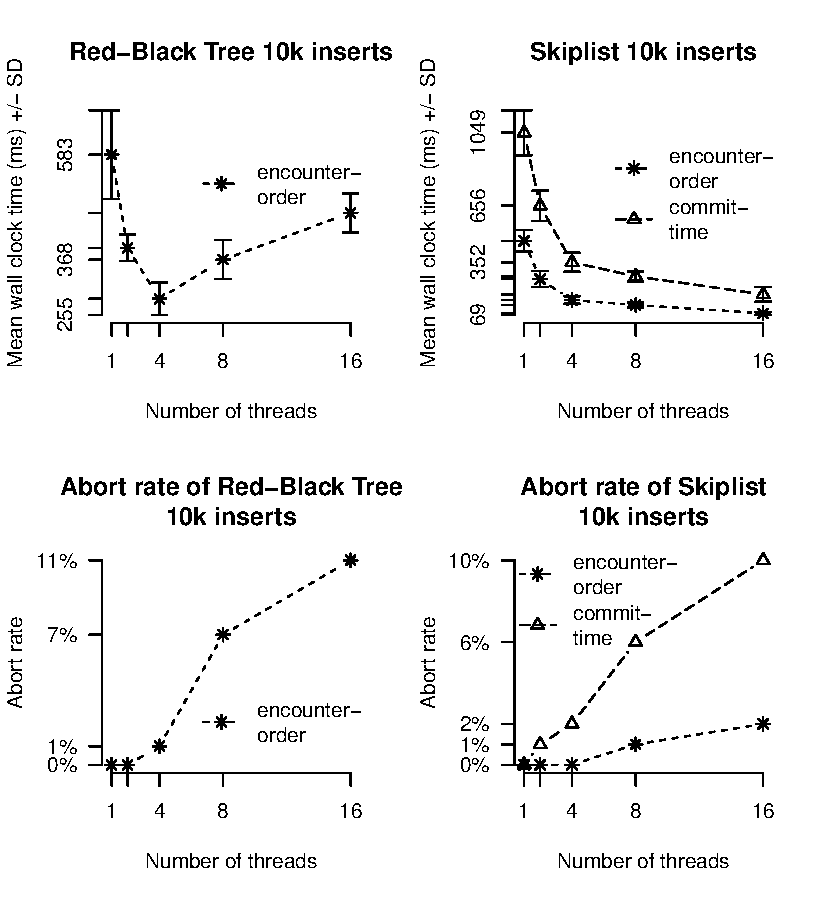
\includegraphics[width=.9\textwidth]{images/plots10k-insert-abort.pdf}}
    \vspace{-0.3cm}
    \caption{Red-Black Tree and Skiplist 10k insertion execution times using encounter-order and commit-time transactions and corresponding abort rates}
    \label{fig:plots10k-insert}
\end{figure}

\begin{figure}[!htb]
    \centering
    \makebox[\textwidth][c]{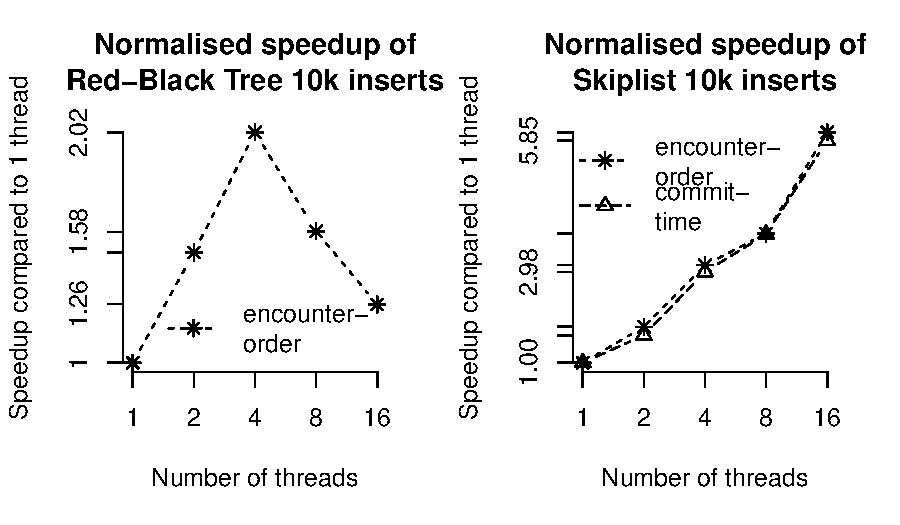
\includegraphics[width=.9\textwidth]{images/plots10k-speedup.pdf}}
    \vspace{-0.3cm}
    \caption{Red-Black Tree and Skiplist 10k insertions speedup compared to sequential execution time}
    \label{fig:plots10k-speedup}
\end{figure}

The relative execution times of the certain operations in the transactional API plotted in Figure \ref{fig:op-times}, provides no surprises, as by analysing the complexities of the algorithms described in Sections \ref{subsection:etx} and \ref{subsection:ctx}, one could have already anticipated the results. 

For the encounter-order algorithm, the \texttt{write()} operation clearly takes up more than half of all the combined execution times as it is responsible for read-set validation, lock acquisition and the atomic stores as well. Following it, the \texttt{commit()} method is the second most costly, responsible for the read-set validation and state reset. The \texttt{abort()} method takes up $7\%$ of all execution times, which is responsible for atomically storing back the original values for the locations. The \texttt{begin()} and \texttt{read()} methods have negligible time complexities, comprised mostly of simple statements and an atomic load in case of the read method. 

For the commit-time algorithm, as one could have expected, it is the \texttt{commit()} method that takes up most of the execution time. It is responsible for lock acquisition, which, due to the existence of the read-set, is in $\mathcal{O}\text{(}n^2\text{)}$; moreover, the read-set validation and atomic stores. Following are the \texttt{write()}, and \texttt{read()} methods, which both need to traverse the write-set to check whether the location is already contained and update the value or return the stored value, respectively. The methods for \texttt{begin()} and \texttt{abort()} have negligible impact on performance, as they consist mostly of simple statements of assignments.

\begin{figure}[!htb]
    \centering
    \makebox[\textwidth][c]{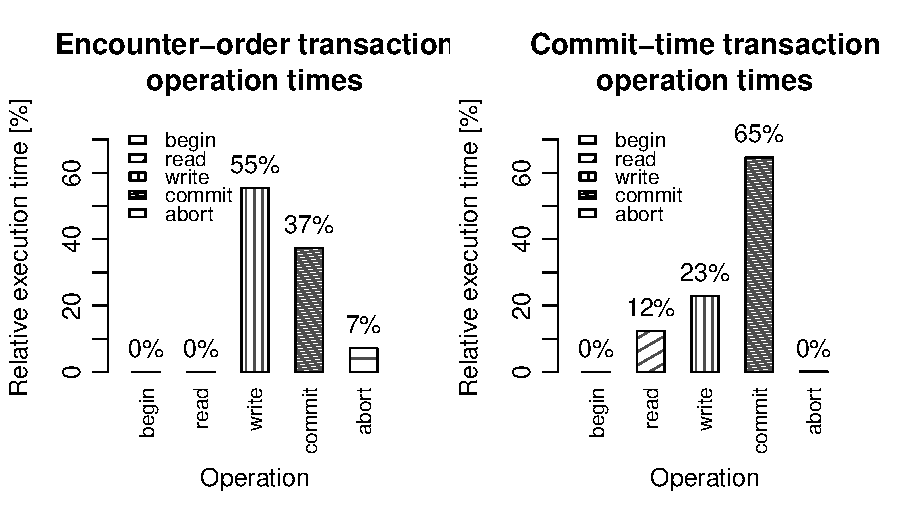
\includegraphics[width=.9\textwidth]{images/op-times.pdf}}
    \caption{Relative operation times of encounter-order and commit-time transactions}
    \label{fig:op-times}
\end{figure}

\section{Discussion}

The performance of the Red-Black Tree is not ideal, as it does not scale well to highly concurrent applications. The suboptimal scaling properties can be largely attributed to the complexity of the Red-Black Tree insertion procedure, which potentially involves a large (and initially unknown) amount of rotations and recolouring, which increases to a great extent the probability of an invalid read-set and hence the rate of aborts. This can also be confirmed by looking at the second plot in the first column of Figure \ref{fig:plots10k-insert} where the abort rate of the encounter-order algorithm is plotted.

As the encounter-order algorithm described in Section \ref{subsection:etx} is similar in nature to the STM proposed by Ennals\cite{ennals-stm}, these findings are in line with what is described by Dice and Shavit in their paper detailing the TL algorithm\cite{tl}, where the performance of encounter-order algorithms are compared. In that paper, the Red-Black Tree test using Ennals' STM version exhibited very similar properties and patterns to what is described in the previous section, matching even the infliction point at $x = 4$.

In the case of the Skiplist, the encounter-order algorithm outperforms the commit-time with about a factor of two in mean wall-clock time and with a factor of 5 in abort rate, even though the achieved speedup was relatively similar for both. This is not in line with the findings of other papers like \cite{tl, tl2}, where it is concluded that commit-time locking should be utilised in case of high contention. However, it can easily be seen that in case of high contention, the abort rate of the commit-time algorithm would drastically increase since there is a very high chance that the read-set is invalidated. This can be further confirmed by looking at the last plot of the second column, where the abort rates are plotted. In the case of executing on 16 threads, there is a difference of a factor of 5 between the abort rate of the encounter order and commit-time locking mechanisms. Encounter-order locking is considered to be a disadvantage by \cite{tl, tl2} as it holds onto locks for a much longer time. However, precisely because of this property, it has a much lower chance of aborting and could still achieve a better performance in the experiment. Moreover, the commit-time algorithm contains a lookaside into the write- and read-sets during committing, as explained in Section \ref{subsection:ctx}, which has $\mathcal{O}(n^2)$ complexity, and its read algorithm has linear time complexity. Compared to the encounter-order algorithm, which has $\mathcal{O}(1)$ read and linear time commit complexities, it is easy to see how it can overperform the commit-time version. We can conclude that the disadvantage of the encounter-order algorithm, namely that it holds onto locks for a much longer time, is still preferable to the complexities introduced in the commit-time algorithm in high-contention situations.